%
% Copyright 2018 Joel Feldman, Andrew Rechnitzer and Elyse Yeager.
% This work is licensed under a Creative Commons Attribution-NonCommercial-ShareAlike 4.0 International License.
% https://creativecommons.org/licenses/by-nc-sa/4.0/
%
\questionheader{ex:s2.13}

%%%%%%%%%%%%%%%%%%
\subsection*{\Conceptual}
%%%%%%%%%%%%%%%%%%

\begin{Mquestion}
Suppose a particular caribou has a top speed of 70 kph, and in one year it migrates 5000 km. What do you know about the amount of time the caribou spent travelling during its migration?
\end{Mquestion}
\begin{hint}
How long would it take the caribou to travel 5000 km, travelling at its top speed?
\end{hint}
\begin{answer}
The caribou spent \emph{at least} about 71 and a half hours travelling during its migration (probably much more) in one year.
\end{answer}
\begin{solution}
We know the top speed of the caribou, so we can use this to give the \emph{minimum} possible number of hours the caribou spent travelling during its migration. If the caribou travels at 70kph, it will take $(5000 \mathrm{km})\left(\dfrac{1 \mathrm{hr}}{70 \mathrm{km}}\right) \approx 71.4 \mathrm{hrs}$ to travel 5000 kilometres. Probably the caribou wasn't sprinting the whole time, so probably it took it longer than that, but we can only say for sure that the caribou spent \emph{at least} about 71.4 hours migrating.
\end{solution}

\begin{Mquestion}
Suppose a migrating sandhill crane flew 240 kilometres in one day. What does the mean value theorem tell you about its speed during that day?
\end{Mquestion}
\begin{hint}
Let $f(x)$ be the position of the crane, where $x$ is the hour of the day.
\end{hint}
\begin{answer}
At some point during the day, the crane was travelling at exactly 10 kph.
\end{answer}
\begin{solution}
If $f(x)$ is the position of the crane at time $x$, measured in hours, then (if we let $x=0$ be the beginning of the day) we know that $f(24)-f(0)=240$. Since $f(x)$ is the position of the bird, $f(x)$ is continuous and differentiable. So, the MVT says there is a $c$ in $(0,24)$ such that $f'(x)=\dfrac{f(24)-f(0)}{24-0}=\dfrac{240}{24}=10$. That is, at some point $c$ during the day, the speed of the crane was exactly 10 kph.
\end{solution}


\begin{Mquestion}
Below is the graph of $y=f(x)$, where $x$ is continuous on $[a,b]$ and differentiable on $(a,b)$. Mark on the graph the approximate location of a value $c$ guaranteed by the mean value theorem.
\begin{center}\begin{tikzpicture}
\YEaaxis{1}{12}{3.5}{3.5}
\draw plot[domain=2:10, samples=100](\x,{(6/(cosh(\x-3))-3});
\draw (2,0.89) node[vertex]{};
\draw (10,-3) node[vertex]{};
\draw (2,.2)--(2,-.2) node[below]{$a$};
\draw (10,.2)--(10,-.2) node[below]{$b$};
\end{tikzpicture}\end{center}
\end{Mquestion}
\begin{hint}
For an example, look at Figure~\ref*{fig rolle_to_mvt}.
\end{hint}
\begin{answer}
One possible answer:
\begin{center}\begin{tikzpicture}
\YEaaxis{1}{12}{3.5}{3.5}
\draw plot[domain=2:10, samples=100](\x,{(6/(cosh(\x-3))-3});
\draw (2,0.89) node[vertex](a){};
\draw (10,-3) node[vertex](b){};
\draw (2,.2)--(2,-.2) node[below]{$a$};
\draw (10,.2)--(10,-.2) node[below]{$b$};
\draw[blue, dashed] (a)--(b);
\draw[red] (3.1,2.95) node[vertex](c1){};
\draw[red, dashed] plot[domain=1:6](\x,{-0.49*\x+4.5});
\draw[red, thick] (3.1,.2)--(3.1,-.2) node[below]{$c$};
\end{tikzpicture}\end{center}
Another possible answer:
\begin{center}\begin{tikzpicture}
\YEaaxis{1}{12}{3.5}{3.5}
\draw plot[domain=2:10, samples=100](\x,{(6/(cosh(\x-3))-3});
\draw (2,0.89) node[vertex](a){};
\draw (10,-3) node[vertex](b){};
\draw (2,.2)--(2,-.2) node[below]{$a$};
\draw (10,.2)--(10,-.2) node[below]{$b$};
\draw[blue, dashed] (a)--(b);
\draw[red, dashed] plot[domain=4:9](\x,{-0.49*\x+.5});
\draw[red] (6.2,-2.55) node[vertex](c2){};
\draw[red] (6.2,.2)--(6.2,-.2) node[below]{$c$};
\end{tikzpicture}\end{center}
\end{answer}
\begin{solution}
The MVT guarantees there is some point $c$ strictly between $a$ and $b$ where the tangent line to $f(x)$ at $x=c$ has the same slope as the secant line of $f(x)$ from $x=a$ to $x=b$. So, let's start by drawing in the secant line.
\begin{center}\begin{tikzpicture}
\YEaaxis{1}{12}{3.5}{3.5}
\draw plot[domain=2:10, samples=100](\x,{(6/(cosh(\x-3))-3});
\draw (2,0.89) node[vertex](a){};
\draw (10,-3) node[vertex](b){};
\draw (2,.2)--(2,-.2) node[below]{$a$};
\draw (10,.2)--(10,-.2) node[below]{$b$};
\draw[blue, dashed] (a)--(b);
\end{tikzpicture}\end{center}
What we're looking for is a point on the curve where the tangent line is parallel to this secant line. In fact, there are two.
\begin{center}\begin{tikzpicture}
\YEaaxis{1}{12}{3.5}{3.5}
\draw plot[domain=2:10, samples=100](\x,{(6/(cosh(\x-3))-3});
\draw (2,0.89) node[vertex](a){};
\draw (10,-3) node[vertex](b){};
\draw (2,.2)--(2,-.2) node[below]{$a$};
\draw (10,.2)--(10,-.2) node[below]{$b$};
\draw[blue, dashed] (a)--(b);
\draw[red] (3.1,2.95) node[vertex](c1){};
\draw[red, dashed] plot[domain=1:6](\x,{-0.49*\x+4.5});
\draw[red, dashed] plot[domain=4:9](\x,{-0.49*\x+.5});
\draw[red] (6.2,-2.55) node[vertex](c2){};
\end{tikzpicture}\end{center}

So, either of the two values  $c_1$ and $c_2$ marked below can serve as the point guaranteed by the MVT:
\begin{center}\begin{tikzpicture}
\YEaaxis{1}{12}{3.5}{3.5}
\draw plot[domain=2:10, samples=100](\x,{(6/(cosh(\x-3))-3});
\draw (2,0.89) node[vertex](a){};
\draw (10,-3) node[vertex](b){};
\draw (2,.2)--(2,-.2) node[below]{$a$};
\draw (10,.2)--(10,-.2) node[below]{$b$};
\draw[blue, dashed] (a)--(b);
\draw[red] (3.1,2.95) node[vertex](c1){};
\draw[red, dashed] plot[domain=1:6](\x,{-0.49*\x+4.5});
\draw[red, dashed] plot[domain=4:9](\x,{-0.49*\x+.5});
\draw[red] (6.2,-2.55) node[vertex](c2){};
\draw[red] (3.1,.2)--(3.1,-.2) node[below]{$c_1$};
\draw[red] (6.2,.2)--(6.2,-.2) node[below]{$c_2$};
\end{tikzpicture}\end{center}
\end{solution}


\begin{question}
Give a function $f(x)$ with the properties that:
\begin{itemize}
\item $f(x)$ is differentiable on the open interval $0<x<10$
\item $f(0)=0$, $f(10)=10$
\end{itemize}
but for all $c \in (0,10)$, $f'(c)=0$.
\end{question}
\begin{hint}
How does this question differ from the statement of the mean value theorem?
\end{hint}
\begin{answer}
One possible answer: $f(x) = \left\{\begin{array}{lr}
0&x \neq 10\\
10&x=10
\end{array}\right.$

Another answer:
$f(x) = \left\{\begin{array}{lr}
10&x \neq 0\\
0&x=0
\end{array}\right.$


Yet another answer:
$f(x) = \left\{\begin{array}{ll}
5&x \neq 0,~10\\
10&x= 10\\
0&x=0
\end{array}\right.$
\end{answer}
\begin{solution}
Since $f(x)$ is differentiable for all $x \in (0,10)$, then $f(x)$ is also continuous for all $x \in (0,10)$. If $f(x)$ were continuous on the closed interval $[0,10]$, then the MVT would guarantee $f'(x)=\dfrac{f(10)-f(0)}{10-0}=1$ for some $c \in (0,10)$; however, this is not the case. So, it must be that $f(x)$ is continuous for all $x \in (0,10)$, but not for all $x \in [0,10]$.

Since $f'(c)=0$ for $c \in (0,10)$, that means $f$ is constant on that interval. So, $f(x)$ is a function like this:
\begin{center}\begin{tikzpicture}
\YEaaxis{1}{5}{1}{5}
\draw node[vertex]{};
\draw (5,5) node[vertex]{};
\draw (0,3) node[opendot]{}--(5,3) node[opendot]{};
\end{tikzpicture}\end{center}
where the height of the constant function can be anything.

So, one possible answer is $f(x) = \left\{\begin{array}{lr}
0&x \neq 10\\
10&x=10
\end{array}\right.$.
\end{solution}


\begin{Mquestion}
For each of the parts below, sketch a function $f(x)$ (different in each part) that is continuous and differentiable over all real numbers, with $f(1)=f(2)=0$, and with
the listed property, or explain why no such function exists.
\begin{enumerate}[(a)]
\item $f'(c)=0$ for \emph{no} point $c \in (1,2)$
\item $f'(c)=0$ for \emph{exactly one} point $c \in (1,2)$
\item $f'(c)=0$ for \emph{exactly five} points $c \in (1,2)$
\item $f'(c)=0$ for \emph{infinitely many} points $c \in (1,2)$
\end{enumerate}
\end{Mquestion}
\begin{hint}
\end{hint}
\begin{answer}
(a) No such function is possible: Rolle's Theorem guarantees $f'(c)=0$ for at least one point $c \in (1,2)$.

For the other functions, examples are below, but many answers are possible.

\begin{center}
\begin{tikzpicture}
\YEaaxis{1}{3}{1}{2}
\draw (.5,0) node[vertex, label=below:1]{};
\draw (2.5,0) node[vertex, label=below:2]{};
\draw[thick] plot[domain=.5:2.5](\x,{-.5*(4*\x*\x-12*\x+5)});
\draw (-1,3) node{(b)};
\end{tikzpicture}
\hfill%
\begin{tikzpicture}
\YEaaxis{1}{4}{1}{2}
\draw (.62,0) node[vertex, label=below:1]{};
\draw (3.76,0) node[vertex, label=below:2]{};
\draw[thick] plot[domain=.62:3.76, samples=100](\x,{-sin(\x*5 r)});
\draw (-1,3) node{(c)};
\end{tikzpicture}
\hfill%
\begin{tikzpicture}
\YEaaxis{1}{3}{1}{2}
\draw (.5,0) node[vertex, label=below:1]{};
\draw (2.5,0) node[vertex, label=below:2]{};
\draw[ultra thick] (.5,0)--(2.5,0);
\draw (-1,3) node{(d)};
\end{tikzpicture}
\end{center}
\end{answer}
\begin{solution}
(a) No such function is possible: Rolle's Theorem guarantees $f'(c)=0$ for at least one point $c \in (1,2)$.

For the other functions, examples are below, but many answers are possible.

\begin{center}
\begin{tikzpicture}
\YEaaxis{1}{3}{1}{2}
\draw (.5,0) node[vertex, label=below:1]{};
\draw (2.5,0) node[vertex, label=below:2]{};
\draw[thick] plot[domain=.5:2.5](\x,{-.5*(4*\x*\x-12*\x+5)});
\draw (-1,3) node{(b)};
\end{tikzpicture}
\hfill%
\begin{tikzpicture}
\YEaaxis{1}{4}{1}{2}
\draw (.62,0) node[vertex, label=below:1]{};
\draw (3.76,0) node[vertex, label=below:2]{};
\draw[thick] plot[domain=.62:3.76, samples=100](\x,{-sin(\x*5 r)});
\draw (-1,3) node{(c)};
\end{tikzpicture}
\hfill%
\begin{tikzpicture}
\YEaaxis{1}{3}{1}{2}
\draw (.5,0) node[vertex, label=below:1]{};
\draw (2.5,0) node[vertex, label=below:2]{};
\draw[ultra thick] (.5,0)--(2.5,0);
\draw (-1,3) node{(d)};
\end{tikzpicture}
\end{center}
\end{solution}



\begin{question}
Suppose you want to show that a point exists where the function $f(x)=\sqrt{|x|}$ has a tangent line with slope $\frac{1}{13}$.
Find the mistake(s) in the following work, and give a correct proof.
\begin{quote}
The function $f(x)$ is continuous and differentiable over all real numbers, so the mean value theorem applies. $f(-4)=2$ and $f(9)=3$, so by the mean value theorem, there exists some $c \in (-4,9)$ such that
$f'(x) = \dfrac{3-2}{9-(-4)}=\dfrac{1}{13}$.
\end{quote}
\end{question}
\begin{hint}
Where is $f(x)$ differentiable?
\end{hint}
\begin{answer}
The function $f(x)$ is continuous over all real numbers, but it is only differentiable when $x \neq 0$. So, if we want to apply the MVT, our interval must consist of only positive numbers or only negative numbers: the interval $(-4,13)$ is not valid.

It is possible to use the mean value theorem to prove what we want: if $a=1$ and $b=144$, then $f(x)$ is differentiable over the interval $(1,144)$ (since 0 is not contained in that interval), and $f(x)$ is continuous everywhere, so by the mean value theorem there exists some point $c$ where $f'(x)=\dfrac{\sqrt{|144|}-\sqrt{|1|}}{144-1}=\dfrac{11}{143}=\dfrac{1}{13}$.

That being said, an easier way to prove that a point exists is to simply find it--without using the MVT. When $x>0$, $f(x)=\sqrt{x}$, so $f'(x)=\dfrac{1}{2\sqrt {x}}$. Then $f'\left(\dfrac{169}{4}\right)=\dfrac{1}{13}$.
\end{answer}
\begin{solution}
The function $f(x)$ is continuous over all real numbers, but it is only differentiable when $x \neq 0$. So, if we want to apply the MVT, our interval must consist of only positive numbers or only negative numbers: the interval $(-4,13)$ is not valid.

It is possible to use the mean value theorem to prove what we want: if $a=1$ and $b=144$, then $f(x)$ is differentiable over the interval $(1,144)$ (since 0 is not contained in that interval), and $f(x)$ is continuous everywhere, so by the mean value theorem there exists some point $c$ where $f'(x)=\dfrac{\sqrt{|144|}-\sqrt{|1|}}{144-1}=\dfrac{11}{143}=\dfrac{1}{13}$.

That being said, an easier way to prove that a point exists is to simply find it--without using the MVT. When $x>0$, $f(x)=\sqrt{x}$, so $f'(x)=\dfrac{1}{2\sqrt {x}}$. Then $f'\left(\dfrac{169}{4}\right)=\dfrac{1}{13}$.
\end{solution}


%%%%%%%%%%%%%%%%%%
\subsection*{\Procedural}
%%%%%%%%%%%%%%%%%%

\begin{Mquestion}[2015Q] Let $f(x)=x^2-2\pi x+ \cos(x)-1$. Show that there exists a real number $c$ such that $f'(c)=0$.
\end{Mquestion}
\begin{hint} To use Rolle's Theorem, you will want two values where the function is zero. If you're stuck finding one of them, think about when $x^2-2\pi x$ is equal to zero.
\end{hint}
\begin{answer} We note that $f(0)=f(2\pi)=0$. Then using the Mean Value Theorem (note that the function is differentiable for all real numbers), we conclude that there exists $c$ in $(0,2\pi)$ such that
$$f'(c)=\frac{f(2\pi)- f(0)}{2\pi - 0} = 0.$$
\end{answer}
\begin{solution} We note that $f(0)=f(2\pi)=0$. Then using the Mean Value Theorem (note that the function is differentiable for all real numbers), we conclude that there exists $c$ in $(0,2\pi)$ such that
$$f'(c)=\frac{f(2\pi)- f(0)}{2\pi - 0} = 0.$$
\end{solution}



\begin{question}[2015Q]
Let $f(x)=e^x + (1-e)x^2 - 1$. Show that there exists a real number $c$ such that $f'(c)=0$.
\end{question}
\begin{answer}
We note that $f(0)=f(1)=0$. Then using the Mean Value Theorem (note that the function is differentiable for all real numbers), we get that there exists $c\in (0,1)$ such that
$$f'(c)=\frac{f(1)- f(0)}{1 - 0} = 0.$$
\end{answer}
\begin{solution}
We note that $f(0)=f(1)=0$. Then using the Mean Value Theorem (note that the function is differentiable for all real numbers), we get that there exists $c\in (0,1)$ such that
$$f'(c)=\frac{f(1)- f(0)}{1 - 0} = 0.$$
\end{solution}


\begin{question}[2015Q]
Let $f(x)=\sqrt{3 + \sin(x)} + (x - \pi)^2$. Show that there exists a real number $c$ such that $f'(c)=0$.
\end{question}
\begin{answer}
We note that $f(0)=f(2\pi)=\sqrt{3} + \pi^2$. Then using the Mean Value Theorem (note that
the function is differentiable for all real numbers since $3+\sin x>0$), we get that
there exists $c\in (0,2\pi)$ such that
$$f'(c)=\frac{f(2\pi)- f(0)}{2\pi - 0} = 0.$$
\end{answer}
\begin{solution}
We note that $f(0)=f(2\pi)=\sqrt{3} + \pi^2$. Then using the Mean Value Theorem (note that
the function is differentiable for all real numbers since $3+\sin x>0$), we get that
there exists $c\in (0,2\pi)$ such that
$$f'(c)=\frac{f(2\pi)- f(0)}{2\pi - 0} = 0.$$
\end{solution}


\begin{question}[2015Q]
Let $f(x)=x\cos(x) - x\sin(x)$. Show that there exists a real number $c$ such
that $f'(c)=0$.
\end{question}
\begin{answer}
We note that $f(0)=0$ and $f(\pi/4)=0$. Then using the Mean Value Theorem (note that the
function is differentiable for all real numbers), we get that there exists $c\in
(0,\pi/4)$ such that
$$f'(c)=\frac{f(\pi/4)- f(0)}{\pi/4 - 0} = 0.$$
\end{answer}
\begin{solution}
We note that $f(0)=0$ and $f(\pi/4)=0$. Then using the Mean Value Theorem (note that the
function is differentiable for all real numbers), we get that there exists $c\in
(0,\pi/4)$ such that
$$f'(c)=\frac{f(\pi/4)- f(0)}{\pi/4 - 0} = 0.$$
\end{solution}




\begin{Mquestion}
How many roots does the function $f(x)=3x-\sin x$ have?
\end{Mquestion}
\begin{hint}
To show that there are exactly $n$ roots, you need to not only show that $n$ exist, but also that there are \emph{not more} than $n$.
\end{hint}
\begin{answer} $1$
\end{answer}
\begin{solution}
By inspection, we see $x=0$ is a root of $f(x)$. The question now is whether there could possibly be other roots. Since $f(x)$ is differentiable over all real numbers, if there is another root $a$, then by Rolle's Theorem, $f'(c)=0$ for some $c$ strictly between $0$ and $a$. However, $f'(x)=3-\cos x$ is never zero. So, there is no second root: $f(x)$ has precisely one root.
\end{solution}




\begin{question}
How many roots does the function $f(x)=\dfrac{(4x+1)^4}{16}+x$ have?
\end{question}
\begin{hint}
To show that there are exactly $n$ roots, you need to not only show that $n$ exist, but also that there are \emph{not more} than $n$.
If you can't explicitly find the root(s), you can use the intermediate value theorem to show they exist.
\end{hint}
\begin{answer}
$2$
\end{answer}
\begin{solution}
The function $f(x)$ is continuous and differentiable over all real numbers.
If $a$ and $b$ are distinct roots of $f(x)$, then $f'(c)=0$ for some $c$ strictly between $a$ and $b$ (Rolle's Theorem). So, let's think about $f'(x)$.
\[f'(x)=(4x+1)^3+1\]
This is simple enough that we can find its zero explicitly:
\[(4x+1)^3 +1= 0
\quad \Leftrightarrow \quad
(4x+1)^3 = -1
\quad \Leftrightarrow \quad
4x+1 = -1
\quad \Leftrightarrow \quad
4x=-2
\]
Hence $f'(c)=0$ only when $c=\dfrac{-1}{2}$. That the derivative only has a single zero is very
useful. It means (via Rolle's theorem) that if $f(x)$ has distinct roots $a$ and $b$ with $a<b$,
then we must have $a < \dfrac{-1}{2} < b$.  This also means that $f(x)$ cannot have 3 distinct
roots $a,b$ and (say) $q$ with $a<b<q$, because then Rolle's theorem would imply that $f'(x)$ would
have two zeros --- one between $a$ and $b$ and another between $b$ and $q$.


We've learned that $f(x)$ has at most two roots, and we've learned something about where those roots can exist, if there are indeed two of them. But that means $f(x)$ could have 0, 1, or 2 roots.

%It's not easy to find a root of $f(x)$ by inspection, so let's  use the Intermediate Value Theorem. For the usual values of $x$ we might try, $f(x)$ is positive: for instance, $f(0)=\frac{1}{16}>0$ and $f(-1)=\frac{81}{16}-1>0$.
%Since $f(x)$ is continuous for all real numbers, if we can find $c$ so that $f(c)<0$, then
%we would be able to guarantee the existence of some roots. A reasonable number to try is $\dfrac{-1}{2}$: this is where the function switches from decreasing to increasing. Indeed,
%\[f\left(\frac{-1}{2}\right)=\frac{1}{16}-\frac{1}{2}<0\]
%Since $f(-1)>0$ and $f\left(\frac{-1}{2}\right)<0$, and since $f$ is continuous, by the IVT $f(x)$ has a root in $\left(\frac{-1}{2},0\right)$.
%Similarly, since $f(1)>0$ and $f\left(\frac{-1}{2}\right)<0$, and since $f$ is continuous, by the IVT $f(x)$ has a root in $\left(-1,\frac{-1}{2}\right)$. So, $f(x)$ has at least two roots. Combining this with our previous results that $f(x)$ has at most two roots, we conclude $f(x)$ has exactly two roots.

It's not easy to find a root of $f(x)$ by inspection. But we can  get a good enough picture of the graph of $y=f(x)$ to tell exactly how many roots there are, just by exploiting the following properties  of $f(x)$ and $f'(x)$.
\begin{itemize}
\item As $x$ tends to $\pm \infty$, $f(x)$ tends to $+\infty$.
\item The derivative $f'(x)=(4x+1)^3+1$ is negative for $x<-\frac{1}{2}$
and is positive for $x>-\frac{1}{2}$. That is, $f(x)$ is decreasing
for $x<-\frac{1}{2}$ and increasing for  $x>-\frac{1}{2}$.
\item $f\left(-\frac{1}{2}\right)=\frac{1}{16}-\frac{1}{2}<0$.
\end{itemize}
This means the function must look something like the graph below:
\begin{center}
 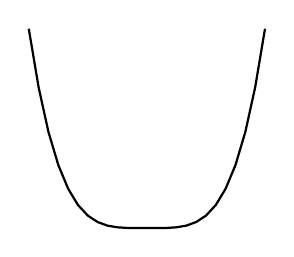
\begin{tikzpicture}
\YEaaxis{3}{2}{1}{2}
\draw[thick] plot[domain=-2:1](\x,{(\x+0.5)*(\x+0.5)*(\x+0.5)*(\x+0.5)*0.5-0.5});
\end{tikzpicture}
\end{center}
except we are unsure of the locations of the $x$-intercepts. At present we only know that one is to
the left of $x=-1/2$ and one is to the right.

Note what happens to $f(x)$ as $x$ increases from strongly negative values to strongly positive
values.
\begin{itemize}
\item When $x$ is large and negative, $f(x)>0$.
\item As $x$ increases, $f(x)$ decreases continuously until
$x=-\frac{1}{2}$, where $f(x)<0$.
 In particular, since $f(-1)=\frac{65}{16}>0$ and
         $f\big(-\frac{1}{2}\big)<0$  and $f(x)$ is continuous,
         the intermediate value theorem guarantees that $f(x)$
         takes the value zero for some $x$ between $-\frac{1}{2}$
         and $-1$.
More descriptively put, as $x$ increases from
hugely negative numbers to $-\frac{1}{2}$, $f(x)$ passes  through zero exactly once.
\item As $x$ increases beyond  $-\frac{1}{2}$, $f(x)$ increases
continuously, starting negative and becoming very large and positive
when $x$ becomes large and positive.
 In particular, since $f(0)=\frac{1}{16}>0$ and
         $f\big(-\frac{1}{2}\big)<0$  and $f(x)$ is continuous,
         the intermediate value theorem guarantees that $f(x)$
         takes the value zero for some $x$ between $-\frac{1}{2}$
         and $0$.
So, as $x$ increases from
$-\frac{1}{2}$ to near $+\infty$, $f(x)$  again passes through
zero exactly once.
\end{itemize}
So $f(x)$ must have exactly two roots, one with $x<-\frac{1}{2}$
and one with $x>-\frac{1}{2}$.
\end{solution}


\begin{question}
How many roots does the function $f(x)=x^3+\sin\left(x^5\right)$ have?
\end{question}
\begin{hint}
If $f(x)=0$, then $|x^3|=\left|\sin\left(x^5\right)\right| \leq 1$. When $|x|<1$, is $\cos(x^5)$ positive or negative?
\end{hint}
\begin{answer}
$1$
\end{answer}
\begin{solution}
\begin{itemize}
\item 
We can see by inspection that $f(0)=0$, so there is at least one root.
We have to determine how many any other roots there are, if any.

\item 
The function $f(x)$ is the sum of the two terms $x^3$ and $\sin(x^5)$. 
A number $x$ is a root of $f(x)$ if and only if the two terms cancel each other exactly for that value of $x$. That is, $x$ is a root of $f$ if and 
only if $x^3=-\sin(x^5)$. To develope some intuition in our hunt for other 
roots, we sketch, in the same figure, the graphs $y=x^3$ and $y=-\sin(x^5)$.
Then the roots of $f(x)$ are precisely the $x$'s where the two curves $y=x^3$ and $y= -\sin(x^5)$ intersect.

\begin{center}
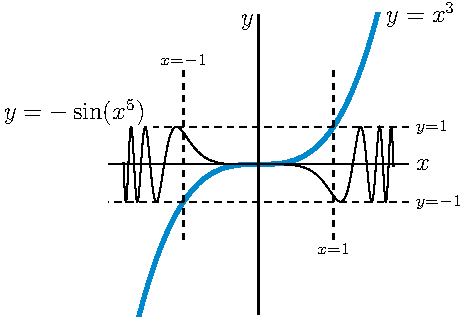
\includegraphics{graphXcubeSin}
\end{center} 

\item Looking at the sketch, we see that the two curves cannot possibly intersect at any point having $|x|>1$ --- if $|x|>1$, then $|x^3|>1$ but
$|-\sin (x^5)|\le 1$ and we cannot possibly have $x^3=-\sin(x^5)$.
That is, all roots of $f(x)$ are in the interval $[-1,1]$. 

\item 
From the sketch, we would probably guess that $y=x^3$ and $y=-\sin(x^5)$ 
cross only at $x=0$. We can use Rolle's Theorem to verify that that is 
indeed the case.

\item If there is a root $a \neq 0$, then by Rolle's Theorem (since $f(x)$ is continuous and differentiable for all real numbers $x$) $f'(c)=0$ for some $c$ strictly between $0$ and $a$. In particular, since we already know any roots $a$ will be between $-1$ and $1$, if $f(x)$ has two roots then $f'(c)=0$ for some $c \in (-1,0) \cup (0,1)$.

\item
The derivative of $f$ is
\begin{equation*}
f'(x)=3x^2+5x^4\cos\big(x^5\big)=x^2\left(3+5x^2\cos\big(x^5\big)\right)
\end{equation*}
So, if $f'(x)=0$, then $x=0$ or $\left(3+5x^2\cos\left(x^5\right)\right)=0$. 
If $x \in (-1,0) \cup (0,1)$, then 
\begin{align*}
|x|<1 &\implies |x^5|<1<\tfrac{\pi}{2}
      \implies \cos\big(x^5\big)>0 \\
      &\implies 3+5x^2\cos\big(x^5\big) > 3 \\
      &\implies f'(x) \neq 0
\end{align*}
That is, there is no $c \in (-1,0) \cup (0,1)$ with $f'(c)=0$. Therefore, following our last  bullet point, $f(x)$ has only one root.
\end{itemize}
Note here that $f'(x)$ has many zeroes --- infinitely many, in fact. However, $x=0$ is the only root of $f'(x)$ in the interval $(-1,1)$.
\end{solution}


\begin{question}
How many positive-valued solutions does the equation $e^x=4\cos(2x)$ have?
\end{question}
\begin{hint}
Let $f(x)=e^x-4\cos(2x)$, and use Rolle's Theorem. What is the interval where $f(x)$ can have a positive root?
\end{hint}
\begin{answer}
$1$
\end{answer}
\begin{solution}

We are to find the number of positive solutions to the equation
          $e^x = 4\cos(2x)$.  The figure below contains the graphs
          of $y=e^x$ and $y= 4\cos(2x)$. The solutions to
          $e^x =  4\cos(2x)$ are precisely the $x$'s where
          $y=e^x$ and $y= 4\cos(2x)$ cross.

\begin{center}
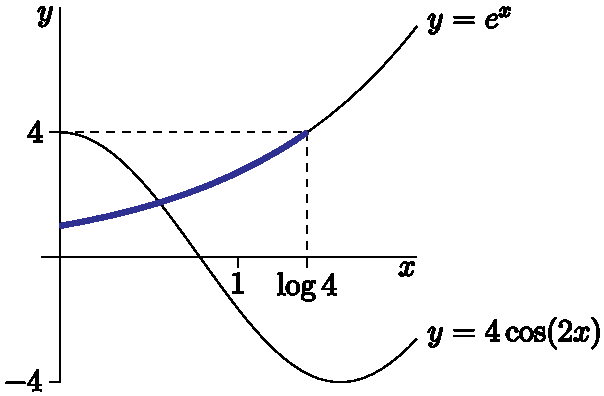
\includegraphics{graphExpCos}
\end{center}

         It sure looks like there is exactly one crossing with $x\ge 0$
         and that one crossing is somewhere between $x=0$ and $x=1$. Indeed
         since $\big[e^x- 4\cos(2x)\big]_{x=0} = -3<0$ and
               $\big[e^x- 4\cos(2x)\big]_{x=1} > e > 0$ and
         $f(x)=e^x- 4\cos(2x)$ is continuous, the intermediate value
         theorem guarantees that there is at least one root with
         $0<x<1$.

         We still have to show that there is no second root --- even if our
         graphs are not accurate.

Recall that the range of the cosine function is $[-1,1]$. If $e^x=4\cos(2x)$, then $e^x \leq 4$, so $x \leq \log(4)\approx 1.39$. So, we only need to search for roots of $f(x)$ on the interval $(0,1.4)$: we are guaranteed there are no roots elsewhere. Over this interval,
$2x \in (0,2.8)$, so $\sin(2x)>0$, and thus $f'(x)=e^x+8\sin(2 x)>0$. Since $f'(x)$ has no roots in $(0,1.4)$, we conclude by Rolle's Theorem that $f(x)$ has at most one root in $(0,1.4)$ (and so at most one positive root total). Since we've already found that a root of $f(x)$ exists in $(0,1)$, we conclude
 $e^x=4\cos(2x)$ has precisely one positive-valued solution.
\end{solution}




\begin{Mquestion}[1997H]
Let $f(x)=3x^5-10x^3+15x+a$, where $a$ is some constant.
\begin{enumerate}[(a)]
\item\label{s2.131997.1}  Prove that, regardless of the value $a$, $f'(x)>0$
for all $x$ in $(-1,1)$.
\item\label{s2.131997.2} Prove that, regardless of the value $a$, $f(x)=3x^5-10x^3+15x+a$
has at most one root in $[-1,1]$.
\end{enumerate}
\end{Mquestion}
\begin{hint} For \eqref{s2.131997.2},  what does Rolle's Theorem tell you has to happen in order for $f(x)$ to have \emph{more than} one root in $[-1,1]$?
\end{hint}
\begin{answer}
\eqref{s2.131997.1} $$
f'(x)=15x^4-30x^2+15=15\big(x^4-2x^2+1\big)=15\big(x^2-1\big)^2\ge 0
$$
The derivative is nonnegative everywhere. The only values of $x$ for which $f'(x)=0$ are $1$ and $-1$, so $f'(x)>0$ for every $x$ in $(-1,1)$.
\smallskip

\eqref{s2.131997.2} If $f(x)$ has two roots $a$ and $b$ in $[-1,1]$, then by Rolle's Theorem, $f'(c)=0$ for some $x$ strictly between $a$ and $b$. But since $a$ and $b$ are in $[-1,1]$, and $c$ is between $a$ and $b$, that means $c$ is in $(-1,1)$; however, we know for every $c$ in $(-1,1)$, $f'(c)>0$, so this can't happen. Therefore, $f(x)$ \emph{does not} have two roots $a$ and $b$ in $[-1,1]$. This means $f(x)$ has at most one root in $[-1,1]$.

\end{answer}
\begin{solution}
\eqref{s2.131997.1} $$
f'(x)=15x^4-30x^2+15=15\big(x^4-2x^2+1\big)=15\big(x^2-1\big)^2\ge 0
$$
The derivative is nonnegative everywhere. The only values of $x$ for which $f'(x)=0$ are $1$ and $-1$, so $f'(x)>0$ for every $x$ in $(-1,1)$.
\smallskip

\eqref{s2.131997.2} If $f(x)$ has two roots $a$ and $b$ in $[-1,1]$, then by Rolle's Theorem, $f'(c)=0$ for some $x$ strictly between $a$ and $b$. But since $a$ and $b$ are in $[-1,1]$, and $c$ is between $a$ and $b$, that means $c$ is in $(-1,1)$; however, we know for every $c$ in $(-1,1)$, $f'(c)>0$, so this can't happen. Therefore, $f(x)$ \emph{does not} have two roots $a$ and $b$ in $[-1,1]$. This means $f(x)$ has at most one root in $[-1,1]$.
\end{solution}


\begin{Mquestion}[2009H]
Find the point promised by the Mean Value Theorem for the function
$e^x$ on the interval $[0, T]$.
\end{Mquestion}
\begin{hint}
Since $f(x)=e^x$ is a continuous and differentiable function, the MVT promises that there exists some number $c$ such that \[f'(c)=\frac{f(T)-f(0)}{T}.\]
Find that $c$, in terms of $T$.
\end{hint}
\begin{answer}
$\log\left(\dfrac{e^T-1}{T}\right)$
\end{answer}
\begin{solution}
Write $f(x)=e^x$. Since $f(x)$ is continuous and differentiable, the Mean Value Theorem asserts that
there exists some $c$ between $0$ and $T$ such that
\begin{align*}
f'(c)&=\frac{f(T)-f(0)}{T-0}
\intertext{The problem asks us to find this value of $c$. Solving:}
 e^c&=\frac{e^T-e^0}{T}\\
e^c&=\frac{e^T-1}{T}\\
 c&=\log\left(\frac{e^T-1}{T}\right)
\end{align*}
\end{solution}


\begin{question}
Use  Corollary~\ref*{cor:DIFFmvtcons} %2.3.11
and Theorem~\ref*{thm:DIFFinvtrigderiv} %2.12.7
in the CLP-1 text to show that $\arcsec x=C-\arccsc x$ for some constant $C$. Find $C$.
\end{question}
\begin{hint}
Let $f(x)=\arcsec x + \arccsc c -C$. %What is the relationship between $\ds\diff{}{x}\arcsec x$ and $\ds\diff{}{x}\{C-\arccsc x\}$?
What is $f'(x)$?
\end{hint}
\begin{answer}
$C=\frac{\pi}{2}$. See the solution for the justification.
\end{answer}
\begin{solution}
The domains of $\arcsec x$ and $C-\arcsec x$ are the same: $|x| \geq 1$.
Define $f(x)=\arcsec x + \arccsc x$, and note that the domain of $f(x)$ is also $|x| \geq 1$.
Using Theorem~\ref*{thm:DIFFinvtrigderiv} in the CLP-1 text,
\begin{equation*}
f'(x)=\diff{}{x}\arcsec x+\diff{}{x} \arccsc x
 = \dfrac{1}{|x|\sqrt{x^2-1}}+\dfrac{-1}{|x|\sqrt{x^2-1}}=0
\end{equation*}
By Corollary~\ref*{cor:DIFFmvtcons} in the CLP-1 text, this means that $f(x)$ 
is constant on any interval in $|x|\ge 1$. So $f(x)$ is a constant, call it $C_+$, on $x\ge 1$, and $f(x)$ is also a constant, call it $C_-$, on $x\le -1$.

In order to find $C_+$, we find $f(1)$, because we know angles for which the secant and cosecant are $x=1$.
\begin{alignat*}{7}
\cos(0)&=1                    &&\implies &\sec(0)&=\tfrac{1}{1}=1 
                              &&\implies &&\arcsec(1)=0
\\
\sin\big(\tfrac{\pi}{2}\big)&=1 
                &&\implies &\csc\big(\tfrac{\pi}{2}\big)&=\tfrac{1}{1}=1 
                &&\implies &&\arccsc(1)=\tfrac{\pi}{2}
\\
        &  && & &  && \implies &&C_+=\arcsec(1)+\arccsc(1)=\tfrac{\pi}{2}
\end{alignat*}
In order to find $C_-$, we find $f(-1)$, because we know angles for which the secant and cosecant are $x=-1$.
\begin{alignat*}{7}
\cos(\pi)&=-1                    &&\implies &\sec(\pi)&=\tfrac{1}{-1}=-1 
                              &&\implies &&\arcsec(-1)=\pi
\\
\sin\big(-\tfrac{\pi}{2}\big)&=-1 
                &&\implies &\csc\big(-\tfrac{\pi}{2}\big)&=\tfrac{1}{-1}=-1 
                &&\implies &&\arccsc(-1)=-\tfrac{\pi}{2}
\\
        &  && & &  && \implies &&C_-=\arcsec(-1)+\arccsc(-1)=\tfrac{\pi}{2}
\end{alignat*}
So $f(x)=\arcsec x + \arccsc x=\frac{\pi}{2}$ for all $|x|\ge 1$
and $\arcsec x = \frac{\pi}{2}- \arccsc x$ for all $|x|\ge 1$.
\end{solution}


%%%%%%%%%%%%%%%%%%
\subsection*{\Application}
%%%%%%%%%%%%%%%%%%


\begin{question}[2009H]
 Suppose $f(0) = 0$ and
$f'(x) = \dfrac{1}{1 + e^{-f(x)}}$ . Prove that $f(100) < 100$.
\medskip

Remark: an equation  relating a function to its own derivative is called a differential equation. We'll see some very basic differential equations in Section~\ref*{sec:ExpGthDecay}.
\end{question}
\begin{hint}
Show that $f$ is differentiable by showing that $f'(x)$ exists for every $x$. Then, the Mean Value Theorem applies. What is the largest $f'(x)$ can be, for any $x$? If $f(100)<100$, what does the MVT tell you must be true of $f'(c)$ for some $c$?
\end{hint}
\begin{answer}
Since $e^{-f(x)}$ is always positive (regardless of the value of $f(x)$),
\[f'(x)=\dfrac{1}{1+e^{-f(x)}}<\dfrac{1}{1+0}=1\] for every $x$.

Since  $f'(x)$ exists for every $x$, we see that $f$ is differentiable, so the Mean Value Theorem applies. If $f(100)$ is greater than or equal to 100, then by the Mean Value Theorem,
 there would have
to be some $c$ between $0$ and $100$ such that
$$
f'(c) = \frac{f(100)-f(0)}{100}\geq\frac{100}{100}= 1
$$

Since $f'(x) \leq 1$ for every $x$, there is \emph{no} value of $c$ as described.
Therefore, it is not possible that  $f(100) \geq 100$. So, $f(100)<100$.
\end{answer}
\begin{solution}
Since $e^{-f(x)}$ is always positive (regardless of the value of $f(x)$),
\[f'(x)=\dfrac{1}{1+e^{-f(x)}}<\dfrac{1}{1+0}=1\] for every $x$.

Since  $f'(x)$ exists for every $x$, we see that $f$ is differentiable, so the Mean Value Theorem applies. If $f(100)$ is greater than or equal to 100, then by the Mean Value Theorem,
 there would have
to be some $c$ between $0$ and $100$ such that
$$
f'(c) = \frac{f(100)-f(0)}{100}\geq\frac{100}{100}= 1
$$

Since $f'(x) < 1$ for every $x$, there is \emph{no} value of $c$ as described.
Therefore, it is not possible that  $f(100) \geq 100$. So, $f(100)<100$.
\end{solution}


\begin{Mquestion}
Let $f(x)=2x+\sin x$. What is the largest interval containing $x=0$ over which  $f(x)$ is one--to--one?  What are the domain and range of $f^{-1}(x)$?
\end{Mquestion}
\begin{hint}
In order for $f^{-1}(x)$ to be defined over an interval, $f(x)$ must be one--to--one over that interval.
\end{hint}
\begin{answer}
Domain of $f^{-1}(x)$: $(-\infty,\infty)$\\
Interval where $f$ is one--to--one, and range of $f^{-1}(x)$: $(-\infty,\infty)$
\end{answer}
\begin{solution}
If $2x+\sin x$ is one--to--one over an interval, it never takes the same value for two distinct numbers in that interval. By Rolle's Theorem, if $f(a)=f(b)$ for distinct $a$ and $b$, then
$f'(c)=0$ for some $c$ between $a$ and $b$. However, $f'(x)=2+\cos x$, which is never zero. In fact, $f'(x)\ge 1$ for all $x$, so $f(x)$ is strictly increasing over its entire domain. Therefore, our function $f$ \emph{never} takes the same value twice, so it is one--to--one over all the real numbers, $(-\infty,\infty)$.

When we define the inverse function $f^{-1}(x)$, the domain of $f$ is the range of $f^{-1}$, and vice-versa. In general, we might have to \emph{restrict} the domain of $f$ (and hence the range of $f^{-1}$) to an interval where $f$ is one--to--one, but in our case, this isn't necessary. So, the range of $f^{-1}$ is $(-\infty,\infty)$ and the domain of $f^{-1}$ is the range of $f$: $(-\infty,\infty)$.
\end{solution}



\begin{question}
Let $f(x)=\dfrac{x}{2}+\sin x$. What is the largest interval containing $x=0$ over which  $f(x)$ is one--to--one?  What are the domain and range of $f^{-1}(x)$, if we restrict $f$ to this interval?
\end{question}
\begin{hint}
In order for $f^{-1}(x)$ to be defined over an interval, $f(x)$ must be one--to--one over that interval.
\end{hint}
\begin{answer}
One--to--one interval, and range of $f^{-1}$: $\left[-\frac{2\pi}{3},\frac{2\pi}{3}\right]$ \\
Domain of $f^{-1}$: $\left[-\left(\frac{\pi}{3}+\frac{\sqrt{3}}{2}\right),\left(\frac{\pi}{3}+\frac{\sqrt{3}}{2}\right)\right]$
\end{answer}
\begin{solution}
If $f(x)=\dfrac{x}{2}+\sin x$ is one--to--one over an interval, it never takes the same value for two distinct numbers in that interval. By Rolle's Theorem, if $f(a)=f(b)$ for distinct $a$ and $b$, then
$f'(c)=0$ for some $c$ between $a$ and $b$. Since $f'(x)=\frac{1}{2}+\cos x$,
$f'(x)=0$ when $x=2n\pi\pm\frac{2\pi}{3}$ for some integer $n$. So, in particular, if  $a$ and $b$ are distinct numbers in the interval $\left[-\frac{2\pi}{3},\frac{2\pi}{3}\right]$, then for every $c$ strictly between $a$ and $b$, $f'(c) \neq 0$, so by Rolle's Theorem $f(a) \neq f(b)$. Therefore $f(x)$ is one--to--one on the interval $\left[-\frac{2\pi}{3},\frac{2\pi}{3}\right]$.

We should also show that the interval $\left[-\frac{2\pi}{3},\frac{2\pi}{3}\right]$ cannot be extended to a larger interval over which $f(x)$ is still one--to--one. %We see that as soon as we let $x$ be a little larger than $\frac{2\pi}{3}$ or a little smaller than $\frac{-2\pi}{3}$, then $f'(x)<0$: so the graph ``reverses direction." % and $f(x)$ repeats values.
Consider the derivative $f'(x) = \frac{1}{2}+\cos x$.
           For all $-\frac{2\pi}{3} < x < \frac{2\pi}{3}$, we have
           $\cos x > -\frac{1}{2}$ (sketch the graph of $\cos x$
           yourself) so that $f'(x)>0$ and $f(x)$ is
           increasing. But at $x=\frac{2\pi}{3}$, $f'(x)=0$, and then
           for $x$ a bit bigger than  $\frac{2\pi}{3}$ we have
           $\cos x < -\frac{1}{2}$ so that $f'(x)<0$ and $f(x)$ is
           decreasing. So the graph ``reverses direction", and $f(x)$
           repeats values. (See the graph of $y=f(x)$ below.) The
           same is true for $x$ a little smaller than $-\frac{2\pi}{3}.$

\begin{center}\begin{tikzpicture}
\YEaxis{3.5}{3.5}
\draw plot[domain=-3.2:3.2](\x,{\x/2+sin(\x r)}) node[right]{$y=f(x)=\dfrac{x}{2}+\sin x$};
\draw (2.1,.2)--(2.1,-.2) node[below]{$\frac{2\pi}{3}$};
\draw (-2.1,.2)--(-2.1,-.2) node[below]{$-\frac{2\pi}{3}$};
\draw (2.1,1.9) node[vertex]{};
\draw (-2.1,-1.9) node[vertex]{};
\end{tikzpicture}\end{center}



When we define the inverse function $f^{-1}(x)$, first we restrict $f$ to $\left[-\frac{2\pi}{3},\frac{2\pi}{3}\right]$. Then the range of $f^{-1}$ is also $\left[-\frac{2\pi}{3},\frac{2\pi}{3}\right]$.  The domain of $f^{-1}$ is the range of $f$ over this interval, so
$\left[-\left(\frac{\pi}{3}+\frac{\sqrt{3}}{2}\right),\left(\frac{\pi}{3}+\frac{\sqrt{3}}{2}\right)\right]$.
\end{solution}


\begin{question}
Suppose $f(x)$ and $g(x)$ are functions that are continuous over the interval $[a,b]$ and differentiable over the interval $(a,b)$. Suppose further that $f(a) < g(a)$ and $g(b)< f(b)$. Show that there exists some $c \in [a,b]$ with $f'(c)>g'(c)$.
\end{question}
\begin{hint}
Let $h(x)=f(x)-g(x)$. What does the Mean Value Theorem tell you about the derivative of $h$?
\end{hint}
\begin{answer}
Define $h(x)=f(x)-g(x)$, and notice $h(a)=f(a)-g(a)<0$ and $h(b)=f(b)-g(b)>0$. Since $h$ is the difference of two functions that are continuous over $[a,b]$ and differentiable over $(a,b)$, also $h$ is continuous over $[a,b]$ and differentiable over $(a,b)$. So, by the Mean Value Theorem, there exists some $c \in (a,b)$ with
\[h'(c)=\frac{h(b)-h(a)}{b-a}\]
Since $(a,b)$ is an interval, $b>a$, so the denominator of the above expression is positive; since $h(b)>0>h(a)$, also the numerator of the above expression is positive. So, $h'(c)>0$ for some $c \in (a,b)$. Since $h'(c)=f'(c)-g'(c)$, we conclude $f'(c)>g'(c)$ for some $c \in (a,b)$.
\end{answer}
\begin{solution}
Define $h(x)=f(x)-g(x)$, and notice $h(a)=f(a)-g(a)<0$ and $h(b)=f(b)-g(b)>0$. Since $h$ is the difference of two functions that are continuous over $[a,b]$ and differentiable over $(a,b)$, also $h$ is continuous over $[a,b]$ and differentiable over $(a,b)$. So, by the Mean Value Theorem, there exists some $c \in (a,b)$ with
\[h'(c)=\frac{h(b)-h(a)}{b-a}\]
Since $(a,b)$ is an interval, $b>a$, so the denominator of the above expression is positive; since $h(b)>0>h(a)$, also the numerator of the above expression is positive. So, $h'(c)>0$ for some $c \in (a,b)$. Since $h'(c)=f'(c)-g'(c)$, we conclude $f'(c)>g'(c)$ for some $c \in (a,b)$.
\end{solution}




\begin{Mquestion}
Suppose $f(x)$ is a function that is differentiable over all real numbers, and $f'(x)$ has precisely two roots. What is the maximum number of distinct roots that $f(x)$ may have?
\end{Mquestion}
\begin{hint}
Rolle's Theorem relates the roots of a function to the roots of its derivative.
\end{hint}
\begin{answer}
$3$
\end{answer}
\begin{solution}
Since $f(x)$ is differentiable over all real numbers, it is also continuous over all real numbers. We claim that $f(x)$ cannot have four or more distinct roots. For every two distinct roots $a<b$, Rolle's Theorem tells us there is a $c \in (a,b)$ such that $f'(c)=0$: that is, $c$ is a root of $f'$. Since $f'$ has only two distinct roots, $f$ can have at most three distinct roots.

\begin{center}
\begin{tikzpicture}
\draw[ultra thick, <->] (0,0)--(6,0);
\color{blue}
\draw (1,.2)--(1,-.2) node[below](a1){$a_1$};
\draw (3,.2)--(3,-.2) node[below](a2){$a_2$};
\draw (5,.2)--(5,-.2) node[below](a3){$a_3$};
\draw (3,-3) node(b){roots of $f(x)$};
\foreach \x in {1,2,3} {\draw[dashed, ->] (b)--(a\x);}
\color{red}
\draw (2,-.2)--(2,.2) node[above](c1){$c_1$};
\draw (4,-.2)--(4,.2) node[above](c2){$c_2$};
\draw (3,3) node(c){roots of $f'(x)$};
\foreach \x in {1,2} {\draw[dashed, ->] (c)--(c\x);}
\end{tikzpicture}\end{center}
\end{solution}



\begin{Mquestion}
How many roots does $f(x)=\sin x + x^2 + 5x +1$ have?
\end{Mquestion}
\begin{hint}
To show that there are exactly $n$ distinct roots, you need to not only show that $n$ exist, but also that there are \emph{not more} than $n$.
\end{hint}
\begin{answer} $2$
\end{answer}
\begin{solution}
We are asked to find the number of solutions to the equation
          $x^2+5x+1 = -\sin x$.  The figure below contains the graphs
          of $y=x^2+5x+1$ and $y=-\sin x$. The solutions to
          $x^2+5x+1 = -\sin x$ are precisely the $x$'s where
          $y=x^2+5x+1$ and $y=-\sin x$ cross.

\begin{center}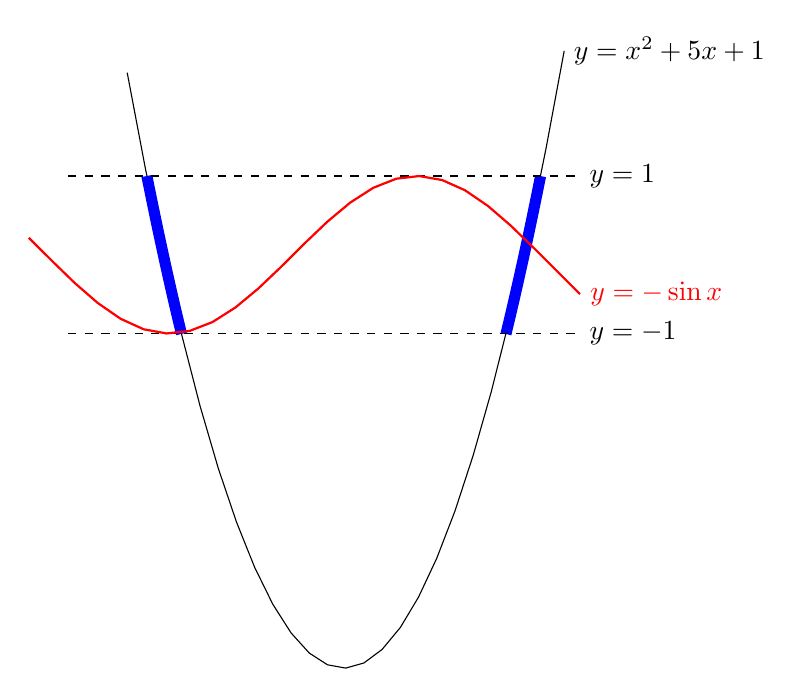
\begin{tikzpicture}
\YEaaxis{7}{2}{5}{3}
\draw plot[domain=-5.25:.3](\x,{\x*\x+5*\x+1}) node[right]{$y=x^2+5x+1$};
\draw[line width=4pt, blue] plot[domain=-5:-4.56](\x,{\x*\x+5*\x+1});
\draw[line width=4pt, blue] plot[domain=-0.44:0](\x,{\x*\x+5*\x+1});
\draw[ dashed] (-6,1)--(.5,1) node[right]{$y=1$};
\draw[ dashed] (-6,-1)--(.5,-1) node[right]{$y=-1$};
\draw[thick, red] plot[domain=-6.5:.5](\x,{-sin \x r}) node[right]{$y=-\sin x$};
\end{tikzpicture}\end{center}


         From the figure, it sure looks like there are two crossings.
         Since the function $-\sin x$ has range $[-1,1]$,
         if the two functions cross, then also $-1 \leq x^2+5x+1\leq 1 $.
         This portion of the quadratic function is highlighted in blue in the figure.
         The $x$ coordinates of the end points
         of the blue arcs are found by solving $x^2+5x+1 = \pm1$,
         i.e. $x=0$, $-5$, and (using the quadratic equation)
         $x= \frac{-5\pm\sqrt{17}}{2}$.

         We are now in a position
         to exploit the intuition that we have built using the above
         figure to write a concise argument showing that $f(x)$ has exactly
         two roots.
         Remember that, in general, if we want to show that a function has $n$ roots, we need to show that there exist $n$ distinct roots somewhere, and that there do not exist $n+1$ distinct roots. This argument is given below, in blue text.
\color{blue}
\begin{itemize}
\item $f(x)$ is continuous over all real numbers
\item $f(x)=0$ only when $-\sin x=x^2+5x+1$, which only happens when $|x^2+5x+1| \leq 1$. Thus, $f(x)$ only has roots in the intervals
$\left[-5,\frac{-5-\sqrt{17}}{2}\right]$ and $\left[\frac{-5+\sqrt{17}}{2},0\right]$.
\item  $f(-5)=\sin(-5)+1 > 0$, and $f\left(\frac{-5-\sqrt{17}}{2}\right)=\sin\left(\frac{-5-\sqrt{17}}{2}\right)-1 <0$.\\ So, by the IVT, $f(c)=0$ for some
$c \in \left(-5,\frac{-5-\sqrt{17}}{2}\right)$.
\item $f(0)=1>0$, and $f\left(\frac{-5+\sqrt{17}}{2}\right)=\sin\left(\frac{-5+\sqrt{17}}{2}\right)-1<0$.\\ So, by the IVT, $f(c)=0$ for some
$c \in \left(\frac{-5+\sqrt{17}}{2},0\right)$.
\item $f'(x)=\cos x + 2x + 5$. If $f'(x)=0$, then $2x+5=-\cos x$, so $|2x+5| \leq 1$. So, the only interval that can contain roots of $f'(x)$ is $[-3,-2]$.
\item Suppose $f(x)$ has more than two roots. Then it has two roots in the interval
$\left[-5,\frac{-5-\sqrt{17}}{2}\right]$ OR it has two roots in the interval
$\left[\frac{-5+\sqrt{17}}{2},0\right]$. Since $f(x)$ is differentiable for all real numbers,  Rolle's Theorem tells us that $f'(x)$ has a root in $\left(-5,\frac{-5-\sqrt{17}}{2}\right)$ or in $\left(\frac{-5+\sqrt{17}}{2},0\right)$. However, since all roots of $f'(x)$ are in the interval $[-3,-2]$, and this interval shares no points with $\left(-5,\frac{-5-\sqrt{17}}{2}\right)$ or $\left(\frac{-5+\sqrt{17}}{2},0\right)$, this cannot be the case. Therefore $f(x)$ does not have more than two roots.
\begin{center}
\begin{tikzpicture}
\draw[ultra thick, <->] (-12,0)--(2,0);
\color{blue}
\draw (-10,.2)--(-10,-.2) node[below]{$-5$};
%\draw (-9,.2)--(-9,-.2) node[below]{$-4.5$};
\draw (-9,.2)--(-9,-.2) node[below]{$\frac{-5-\sqrt{17}}{2}$};
\draw[line width=4pt] (-10,0)--(-9,0);
%\draw (-1,.2)--(-1,-.2) node[below]{$-0.5$};
\draw (-1,.2)--(-1,-.2) node[below]{$\frac{-5+\sqrt{17}}{2}$};
\draw (0,.2)--(0,-.2) node[below]{$0$};
\draw[line width=4pt] (-1,0)--(0,0);
\draw (-5,-3) node(c){roots of $f(x)$};
\draw [dashed, ->] (c)--(-9.5,-1);
\draw [dashed, ->] (c)--(-.5,-1);
\color{red}
\draw (-6,-.2)--(-6,.2) node[above]{$-3$};
\draw (-4,-.2)--(-4,.2) node[above]{$-2$};
\draw[line width=4pt] (-6,0)--(-4,0);
\draw (-5,3) node(d){roots of $f'(x)$};
\draw [dashed, ->] (d)--(-5,1);
\end{tikzpicture}
\end{center}
\item Since $f(x)$ has at least two roots, and not more than two roots, $f(x)$ has exactly two roots.
\end{itemize}

\color{black}


%It's not easy to find a root of $f(x)$ by inspection, but we notice the following:
%\begin{itemize}
%\item $f(x)$ is continuous for all real numbers
%\item $f(0)=1>0$
%\item $f(-\pi)=\pi^2-5\pi+1<0$
%\end{itemize}
%So, by the Intermediate Value Theorem, $f(x)$ has a root in the interval $(-\pi,0)$.
%Now, let's think about the roots of $f'(x)=\cos x + 2x + 5$. This function has at least one root (again, we can use IVT: $f(0)=6>0$, and $f(-\pi)=-2\pi+4<0$) so it's possible that $f(x)$ has two or more roots.
%
%At this point, we don't know much: $f(x)$ has at least one root. If $f'(x)$ were a function with no roots, we'd be done, but such is not the case. So, we decide to be more careful. Rolle's Theorem tells us that, if $f(a)=f(b)=0$ and $a \neq b$, then $f'(c)=0$ for some $c$ strictly between $a$ and $b$. So, let's look at where $f$ and $f'$ could have roots.
%
%If $f(x)=0$, then $x^2+5x+1=-\sin x$, so $|x^2+5x+1| \leq 1$. Let's figure out which values of $x$ this corresponds to. The function $x^2+5x+1$ is an upwards-pointing parabola. $x^2+5x+1=1$ when $x=0$ and $x=-5$, and
% $x^2+5x+1=-1$ when $x=\dfrac{-5\pm\sqrt{17}}{2}$, or  $x \approx -4.56$ and $x \approx -0.44$. Therefore, all roots of $f(x)$ are in the intervals $\left[-5,\dfrac{-5-\sqrt{17}}{2}\right] $ and $\left[\dfrac{-5+\sqrt{17}}{2},0\right]$.
%
%Now, let's consider where $f'(x)$ can be zero. If $0=f'(x)=\cos x + 2x +5$, then $2x+5=\cos x$, so $|2x+5| \leq 1$. Therefore $f'(x)$ only has roots in the interval $[-2,-3,]$.
%By Rolle's Theorem, there can be at most one root of $f(x)$ in the interval $\left[\frac{-5+\sqrt{17}}{2},0\right]$ (otherwise there would be a root of $f'(x)$ in$\left(\frac{-5+\sqrt{17}}{2},0\right)$, which isn't true) and  there can be at most one root of $f(x)$ in the interval $\left[-5,\frac{-5-\sqrt{17}}{2}\right]$ (otherwise there would be a root of $f'(x)$ in $\left(-5,\frac{-5-\sqrt{17}}{2}\right)$ , which isn't true). We already know that $f(0)=0$, so $0$ is the only root of $f(x)$ outside of the interval $\left[-5,\frac{-5-\sqrt{17}}{2}\right]$ . Let's investigate this interval further. At its endpoints: $f(-5)=\sin(-5)+1 > 0$, and $f\left(\frac{-5-\sqrt{17}}{2}\right)=\sin\left(\frac{-5-\sqrt{17}}{2}\right)-1 <0$. So, since $f(x)$ is continuous over all real numbers, by the IVT, $f(x)$ has a root in this interval.
\end{solution}
